\documentclass[12pt]{article}
\usepackage[utf8]{inputenc}
\usepackage[english]{babel}
\usepackage[letterpaper, portrait, margin=1in]{geometry}
\usepackage{amsmath}
\numberwithin{equation}{section}
\usepackage{amssymb}
\usepackage{graphicx}
\usepackage{parskip}
\usepackage{xcolor}
\usepackage{physics}
\usepackage{empheq}
\usepackage{cancel}
\usepackage{hyperref}
\hypersetup{colorlinks = true, urlcolor = blue, linkcolor = red, citecolor = red}
\usepackage{enumerate}
\usepackage{tikz}
\usepackage{float}
\usepackage{tcolorbox}
\usepackage{booktabs}
\usepackage[bottom]{footmisc}
\usepackage{soul}

\usepackage{xcolor}
\usepackage{fancyhdr}
\pagestyle{fancy}
\fancyhf{}
\fancyfoot[C]{\color{lightgray} Statistics Lecture I Notes}
\fancyfoot[L]{\color{lightgray} \today}
\fancyfoot[R]{Page \thepage}
\renewcommand{\headrulewidth}{0pt}
\renewcommand{\footrulewidth}{0pt}

\renewcommand{\arraystretch}{2}

\begin{document}
	
\section{Introduction}

Why do we care about statistic and probability in physics?
\begin{itemize}
	\item Experimental uncertainty: how confident are you about your measurements? Is your experimental data consistent with your model? 
	\item Physics is statistical: statistical mechanics (thermodynamics) and quantum mechanics (statistical ensembles).
\end{itemize}

\section{Events, Sample Spaces, RVs}

\begin{itemize}
	\item EVENT: a possible result of a measurement or experiment. Probability describes the statistics of an event happening.
	\item SAMPLE SPACE: the set of all events. For example, for a coin toss, the event space $ E $ is given by $ E = \{H, T\} $.
	\item RANDOM VARIABLE: a variable that represents the numerical result of a random process.  A RV takes on different values by chance. Each value the RV can take represents an event in the sample space. For example: if $ X $ is the result of a dice roll, then after rolling a 5, the RV has value $ X=5 $
	\item Function of random variables: suppose $ X,Y $ are random variables. We can define another random variable as a function of $ X,Y $,
	\begin{equation}
			Z = f(X,Y)
	\end{equation}
NOTE: the probability distribution of functions of random variables are not trivial. For example, let $ X,Y $ be independent RVs for a coin toss (0 tails, 1 heads) and $ Z = X+Y $.
\begin{align}
	P(Z=0) &= P(X=0\cap Y=0) = 1/4\\
	P(Z=1) &= P(X=0\cap Y=1) + P(X=1\cap Y=0) = 1/2\\
	P(Z=2) &= P(X=1\cap Y=1) = 1/4
\end{align}
In general,
\begin{equation}
		P(Z=n) = \sum_{x,y: f(X=x,Y=y)=n}P(X=x\cap Y=y)
\end{equation}
\end{itemize}

\section{Probability}
\begin{itemize}
	\item For equally likely outcomes, the probability of event $ A $ is,
	\begin{equation}
			P(A) = \frac{\# A}{\# \text{total}}
	\end{equation}
	\item Complements: $ P(A^C)  = 1-P(A)$ (draw diagram)
	\item Union ($ \cup $) and intersection ($ \cap $)
	\item Inclusion-exclusion rule: (for 2 sets)
	\begin{equation}
			P(A \cup B) = P(A) + P(B) - P(A\cap B)
	\end{equation}
	This can be generalized: the cardinality of the union of $ n $ sets:
	\begin{enumerate}
		\item Include the cardinalities of the sets.
		\item Exclude the cardinalities of the pairwise intersections.
		\item Include the cardinalities of the triple-wise intersections.
		\item Exclude the cardinalities of the quadruple-wise intersections.
		\item $ \dots $ continue, until the n-tuple-wise intersection
	\end{enumerate}
	\item Conditional probability: $ P(A\cap B)  = P(A)P(B|A) = P(B)P(A|B)$
	\item Bayes rule (from above):
	\begin{equation}
			P(B|A) = \frac{ P(A\cap B) }{P(A)} = \frac{P(B)P(A|B)}{P(A)} 
	\end{equation}
	\item INDEPENDENCE: if events $ A,B $ are independent,
	\begin{equation}
			P(A\cap B) = P(A)P(B)
	\end{equation}
\end{itemize}

\section{Expectation and uncertainty}
\begin{itemize}
	\item The EXPECTATION value of a RV is the average value of the RV. For RV $ X $,
	\begin{equation}
			E(X) = \sum_{x'} x' P(X=x')
	\end{equation}
	\item Properties:
	\begin{enumerate}
		\item $ E(X+Y)  = E(X) + E(Y)$ where $ X,Y $ do not have to be independent (there's a cool proof just by rearranging terms in the sum \href{https://www.ocf.berkeley.edu/~yizhu/static/notes/stat_134_review.pdf}{pg 6}) 
		\item $ E(a\cdot C)  = a\cdot P(X)$ where $ a $ is a constant.
		\item In general, $ E[f(X,Y)] \neq f(E(Y), E(Y))$. For example, $ E(X\cdot Y)\neq E(X)E(Y) $.
	\end{enumerate}
	\item UNCERTAINTY: Variance is expectation value of the squared deviation from the mean $ \mu $.
	\begin{equation}
			Var(X) = E[(X-\mu)^2] = E(X^2) - [E(X)]^2
	\end{equation}
	Properties of variance:
	\begin{enumerate}
		\item $ Var(a X + b) =a^2\cdot Var(X)$ 
	\end{enumerate}
	In physics, we call the standard deviation the uncertainty,
	\begin{equation}
			SD(x) = \sqrt{Var(X)}
	\end{equation}
\end{itemize}

\section{Distributions}
\begin{itemize}
	\item BERNOULLI trial: tossing a weighted coin with probability $ p $ of getting heads,
	\begin{equation}
			\text{Bernoulli}(p)=\begin{cases}
				1,&p\\
				0,&1-p=q
			\end{cases}
	\end{equation}
	\item BINOMIAL distribution: the probability of $ k $ successes in $ n $ Bernoulli$ (p) $ trials.
	\begin{equation}
			\text{Binomial}(p) = {n \choose k} p^k q^{n-k}
	\end{equation}
	\textit{$ n $ choose $ k $}: the number of ways to choose $ k $ successful trials among $ n $  total trials.
	\begin{equation}
			{n\choose k} = \frac{n!}{k!(n-k)!}
	\end{equation}
	Mean: $ np $, Variance: $ npq $
	\item The binomial theorem:
	\begin{equation}
			(p+q)^n = \sum_{k=0}^\infty {n \choose k} p^k q^{n-k}
	\end{equation}

\item The binomial distribution can be generalized:

\begin{center}

\begin{tabular}{c|c|c}
	& \textbf{2 outcomes per trial} &\textbf{ multiple outcomes per trial}\\
	\midrule
	\shortstack{Independent trials\\(w/replacement)} & binomial & multinomial\\
	\midrule
	\shortstack{Dependent trails\\(wo/replacement)} & hypergeometric & multivariate hypergeometric
\end{tabular}
\end{center}

\item NORMAL distribution. Q: how tall is the Campanille? If I were to give you a meter stick, ladder, and a well-written liability release form, you could measure for yourself! If you were to measure the height 20 times, we would expect a slightly different value each time. If we were to plot the measured values, we would expect a distribution that looks like a normal distribution.

\st{Data is normally distributed if the rate that the probability density falls is proportional to the distance from the mean.} (Almost)
\begin{equation}
		\dv{f}{x} = -k(x-\mu)\quad \Longrightarrow\quad f(x) = -\frac{k}{2}(x-\mu)^2
\end{equation}
The probability density here is a parabola, and will go negative. Instead,

Data is normally distributed if the \textit{rate} that the probability density falls is \textit{proportional} to the distance from the mean \textit{and} the probability density at that location.
\begin{equation}
		\dv{f(x)}{x} = -k(x-\mu) f(x)
\end{equation}
\begin{equation}
		\int \frac{1}{f(x)}	\dv{f(x)}{x}\dd x = \int -k(x-\mu) \dd x
\end{equation}
\begin{equation}
		\ln(f) = -\frac{k}{2}(x-\mu)^2 + \ln(A)
\end{equation}
\begin{equation}
		f(x) = Ae^{-\frac{1}{2}(x-\mu)^2}
\end{equation}
By normalization, we will find,
\begin{equation}
		f(x) = \frac{1}{\sqrt{2\pi}\sigma}e^{-\frac{1}{2}(x-\mu)^2}
\end{equation}
Notice that $ f(x) $ is the probability density function. This means the probability is given by,
\begin{equation}
		P(x\in[x_0, x_1]) = \int_{x_0}^{x_1} f(x)\dd x
\end{equation}
We can say the RV $ X $ is normally distributed with the notation $ X\sim N(\mu, \sigma^2) $
\item Normal approximation to the binomial: for $ n $ sufficiently large, the normal distribution approximates the binomial with mean $ np $ and variance $ npq $.

\begin{figure}[H]
	\centering
	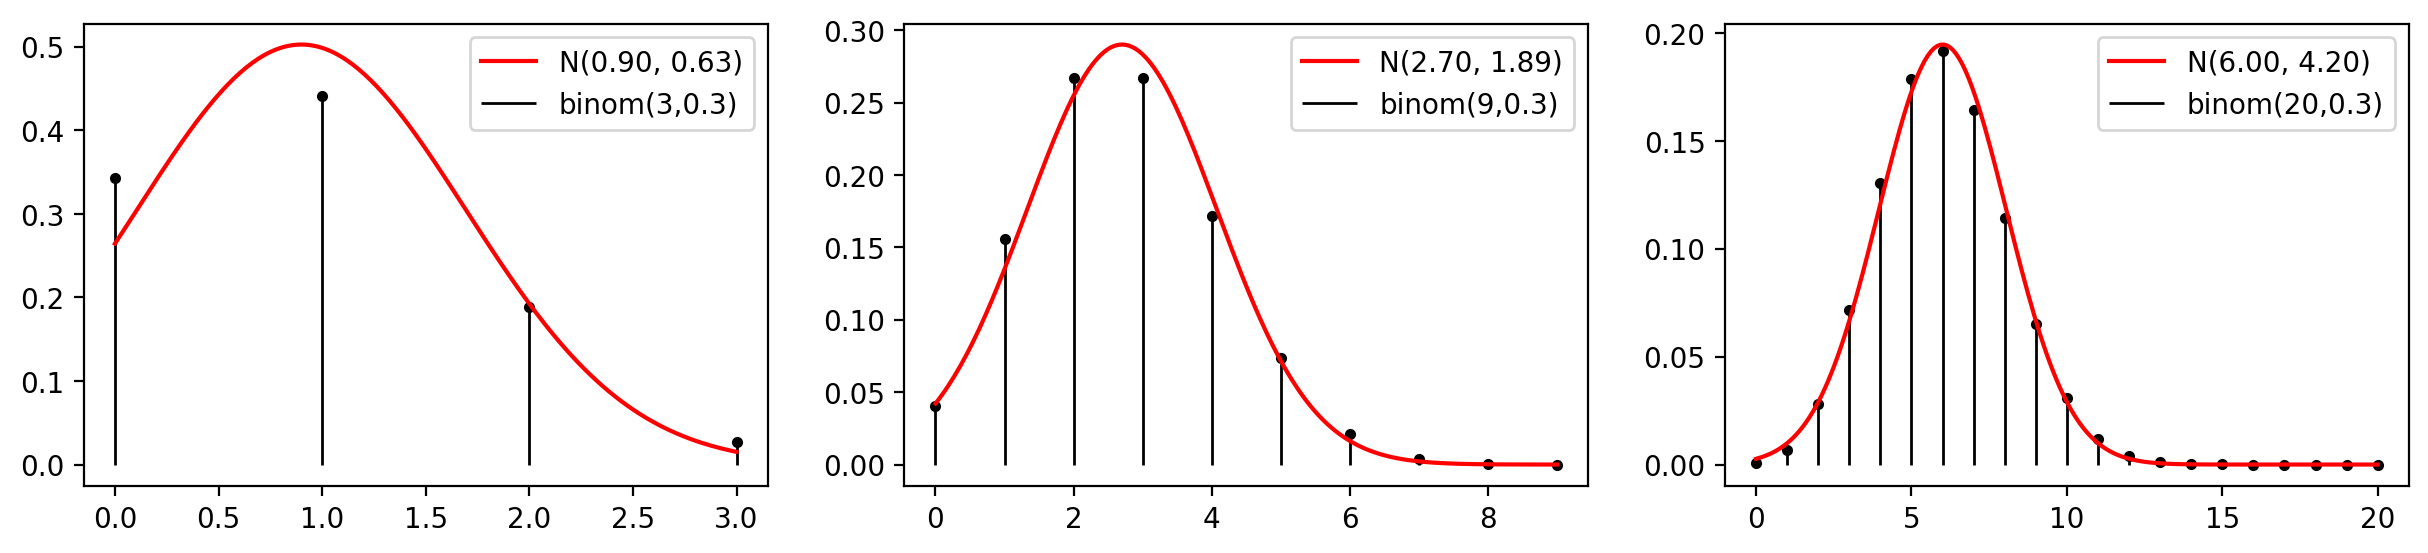
\includegraphics[width=16cm] {binom}
\end{figure}

\item POISSON distribution: A Poisson process is a simple stochastic model for arrivals. What do we mean by arrivals?

Suppose you build a muon detector. For the size of the detector, you expect (i.e. on average) to observe $ \lambda $ arrivals per unit time. If you wait $ t $ seconds: what is the probability distribution of the number of muons you will have observed? This is modeled by the Poisson distribution.

Assumptions:
\begin{enumerate}
	\item The average rate of an event (i.e. an arrival) is $ \lambda $
	\item The events are independent
	\item Two events can not occur at the same time
\end{enumerate}

What is the probability that we observe $ x $ events in time $ t $?

We break up the time $ t $ into $ n $ intervals. For $ n $ large enough (i.e. when we take $ n\to\infty $), the time interval is so short that, at most, one event can occur. The probability of this event occurring is $ \lambda (t/n) $. Therefore, we can model each small time intervals as a Bernoulli trial with $ p=\lambda t/n $ 

\begin{figure}[H]
	\centering
	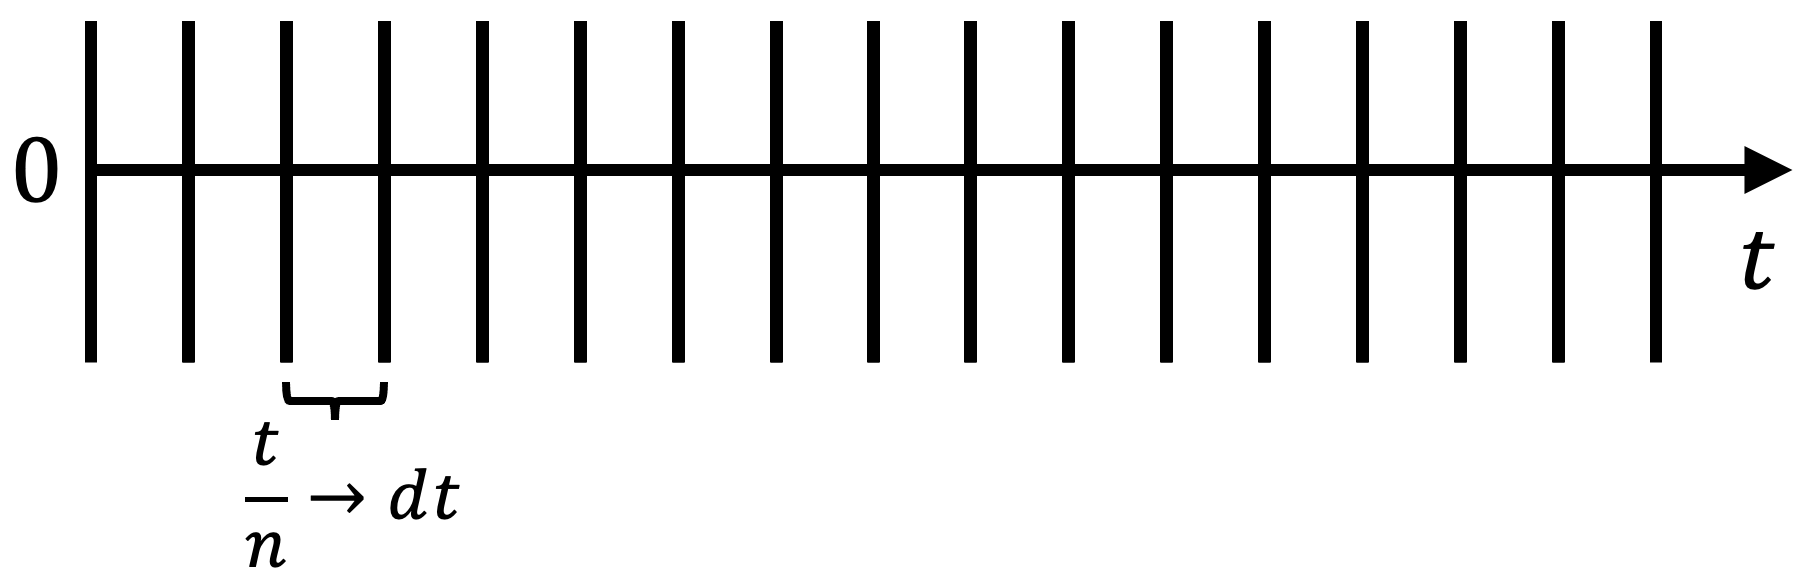
\includegraphics[width=9cm] {poi}
\end{figure}

Then, the probability of $ x $ arrivals is given by the binomial distribution, 
\begin{align}
		P(x \text{ arrivals}) &= \lim_{n\to\infty} {n \choose x} \left(\frac{\lambda t}{n}\right)^x \left(1-\frac{\lambda t}{n}\right)^{n-x}\\
		&= \frac{n!}{x!(n-x)!}\frac{(\lambda t)^x}{n^x}\left(1-\frac{\lambda t}{n}\right)^{n} \cancelto{_1}{\left(1-\frac{\lambda t}{n}\right)^{-x}}\\
		&= \frac{n!}{(n-x)!\ n^x}\frac{(\lambda t)^x}{x!} e^{-\lambda t} \\
		&= \left[\frac{n(n-1)(n-2)\dots (n-x+1)}{n^x}\right]\frac{(\lambda t)^x}{x!}  e^{-\lambda t}\\
		&= \cancelto{_1}{\left[ \frac{n}{n} \cdot \frac{n-1}{n} \cdot \frac{n-2}{n} \cdot \dots \cdot \frac{n-x+1}{n} \right]}\frac{(\lambda t)^x}{x!}  e^{-\lambda t}\\
\end{align}
\begin{equation}
		P(x \text{ arrivals}) = \frac{(\lambda t)^x  e^{-\lambda t}}{x!}
\end{equation}

The mean and variance of Poisson$(\lambda t)  $ is $ \lambda t $

\begin{figure}[H]
	\centering
	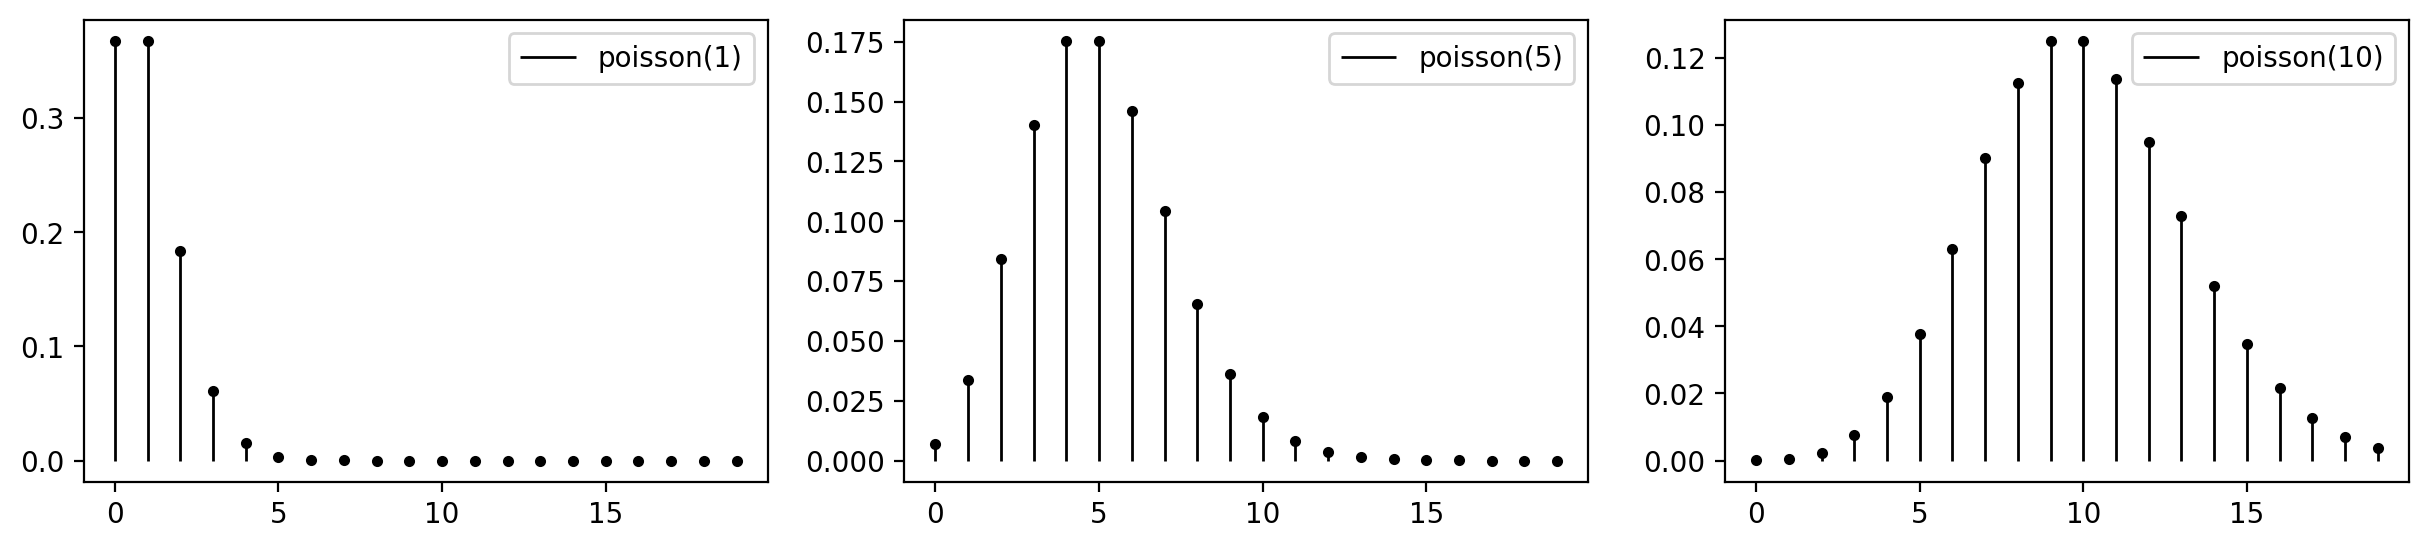
\includegraphics[width=16cm] {poisson}
\end{figure}

\item The Gamma distribution is closely related to the Poisson process. You can read more in a statistics textbook. The GAMMA FUNCTION is derived from the Gamma distribution, and will be relevant when we discus the $ \chi^2 $ distribution.

\item Gamma function:
\begin{equation}
		\Gamma (z) = \int_0^\infty  x^{z-1}e^{-x}\dd x
\end{equation}

For $ z\in \mathbb{N} $, $ \Gamma(z) = (z-1)! $. The Gamma function can be considered an analytic continuation of the factorial to a larger domain.

\end{itemize}

\section{Summary}
\begin{itemize}
	\item Today we discussed a basic summary of the formalism of probability, RVs, and some common distributions.
	\item There is one more important distribution: the $ \chi^2 $ distribution, which we will discuss next week
	\item Next time we will also discuss curve fitting and understanding if a model is a good fit.
\end{itemize}

\end{document}
